\documentclass{article}

% Lenguaje y Fuente
\usepackage[spanish]{babel}
\usepackage[utf8x]{inputenc}
\usepackage[T1]{fontenc}
\usepackage[top=1in, bottom=1.25in, left=1.1 in, right=1.1 in]{geometry}
\usepackage{graphicx}
\usepackage{ragged2e}
\usepackage[usenames]{color}
\usepackage{multicol}

% Portada

\title{\textbf{Reporte de la Actividad 6}\\ Modelo INIFAP-CECH para el cálculo de Horas Frío}
\author{Luis Fernando Duarte Gonzalí \\ Universidad de Sonora \\ Física Computacional}
\date{Marzo del 2019}
\begin{document}
\maketitle

% Contenido del Reporte

\section{Introducción}

\noindent En el siguiente documento se seguirá practicando con la biblioteca Matplotlib de Python para seguir analizando datos, se mostrarán en gráficas de los cálculos obtenidos con el modelo de INIFAP-CECH de Grageda Grageda y colaboradores de 2002 de las Horas de Frío Efectivas. Seguiremos trabajando con el documento de \textit{Vid.dat}, ahora comparándolo con el modelo Utah, desarrollado por Richardson en 1974.

El archivo que se utilizó cuenta con los datos medidos por la estación ubicada en un cultivo de Vid, en el Km. 41 de la carretera Hermosillo a Bahía Kino.

\subsection{Requerimiento de frío en especies frutales caducifolias}

\subsubsection*{Sección tomada de wikipedia}

El requerimiento de frío en especies frutales caducifolias, requisito también conocido como acumulación de frío, es un factor decisivo en la adaptación de estas especies a su ambiente. De este requerimiento depende la ruptura de la dormición de un amplio espectro de árboles y arbustos frutales de uso comercial, tales como las especies frutales de pepita (manzano, peral, membrillero), las de hueso o carozo (duraznero o melocotonero, ciruelo japonés, cerezo dulce, guindo, olivo, etc), las especies productoras de frutos secos (almendro, avellano, nogal, castaño, pecán, pistachero), los arbustos de hoja caduca (arándanos, frambueso, moras, zarzamora, grosellero), y las especies de hoja caduca trepadoras (vid, actinidia). Todas ellas tienen que estar expuestas a un período de bajas temperaturas durante el letargo invernal para una adecuada ruptura de la dormición e inicio de la nueva estación de crecimiento.

Cuando las especies frutales de clima templado no resultan expuestas a temperaturas bajas de acuerdo a sus necesidades específicas (siendo en general la eficiencia máxima entre 2,5 y 9,1 °C), se observan un conjunto de síntomas entre los que resultan más comunes los siguientes:

\begin{itemize}
    \item retraso en la apertura de yemas de madera;
    \item retraso en la apertura de yemas de flor;
    \item brotación irregular y dispersa; y
    \item desprendimiento de las yemas de flor.
\end{itemize}

Consecuentemente, la productividad de la especie se ve seriamente comprometida.

\subsection{Modelo Utah}

Hay varios modelos para realizar el cálculo de horas frío requeridos para cada tipo de especie. La Universidad de California en Davis, tiene un sitio para el cálculo de horas frío y apoyar a los productores utilizando varios modelos. Un modelo muy popular es el modelo Utah desarrollado por Arlo Richardson y colegas en 1974. El modelo Utah de Richardson está resumido en la siguiente tabla: 
\begin{table}[htb]
\centering
\begin{tabular}{ c | c }
\hline
    \multicolumn{2}{ c }{\textbf{Relación de eficacia para la salida de la dormición}(UF denota la Unidad de Frío)} \\ \hline \hline
    \textbf{Temperatura (ºC)} & \textbf{UF correspondientes a 1 hr transcurrida a un dado rango térmico} \\
\hline \hline
    < 1,4 & 0 \\ \hline   
    1.5 a 2.4 & 0.5 \\ \hline
    2.5 a 9.1 & 1.0 \\ \hline
    9.2 a 12.4 & 0.5\\ \hline
    12.5 a 15.9 & 0 \\ \hline
    16.0 a 18.0 & -0.5 \\ \hline 
    > 18.0  & -1.0 \\ \hline 
\end{tabular}
\end{table}
Cada día se suman las unidades de frío y se denotan por UF24. Si vemos un ejemplo del sitio de la Universidad de California, se va sumando cada día las UF24 a partir del 1 de Noviembre para cada cultivo, acumulándose hasta alcanzar el rango de horas frío requeridas para el brote de un cultivo.

\section{Análisis de Datos}
Los datos que contiene el archivo de \textit{Vid.dat} los limitamos para que fueran desde Noviembre del 2018 hasta Febrero del presente año, no contiene ninguna sin datos, es decir, no tiene espacios vacíos entre estas fechas, por lo que tendremos gráficas sin datos nulos. Si es que faltaran datos se podrían interpolar los datos faltantes, pero no es muy recomendable ya que es información casi "inventada", ya que son procesos casi aleatorios, otra técnica sería cortar los datos y no tener gráficas con espacios vacíos por falta de información.

\noindent Para comenzar, necesitamos abrir \textsc{Jupyter Lab} desde Anaconda Prompt, abriendo la carpeta creada previamente con el nombre de \textit{Actividad6}.
Una vez abierto, en python, primero se importaron las bibliotecas Pandas, Numerical Python y Matplot para generar las gráficas.

\begin{center}
    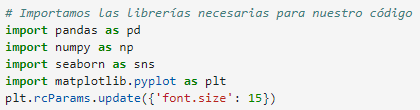
\includegraphics[scale = 0.6]{Images/Import.png}
\end{center}
Luego leémos el archivo previamente mencionado y creamos columnas para hora, dia, mes y año:
\begin{center}
    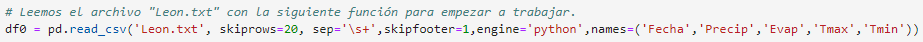
\includegraphics[scale = 0.7]{Images/read.png}
\end{center}
\begin{center}
    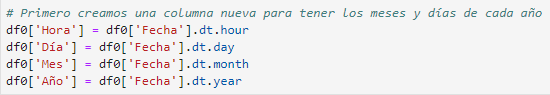
\includegraphics[scale = 0.7 ]{Images/fecha.png}
\end{center}
Agrupamos para sacar los promedios y obtener las columnas de temperaturas máxima y mínima:
\begin{center}
    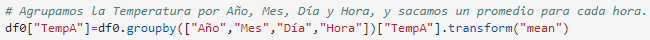
\includegraphics[scale = 0.6]{Images/group.png}
    \\
    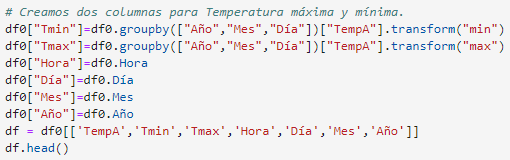
\includegraphics[scale = 0.6]{Images/Temp.png}
\end{center}
\begin{center}

\end{center}

\subsection{Índice UF24}
Se utilizó el siguiente código donde introducimos un \textit{loop} para calcular el índice de Unidades de Frío por día:
\begin{center}
    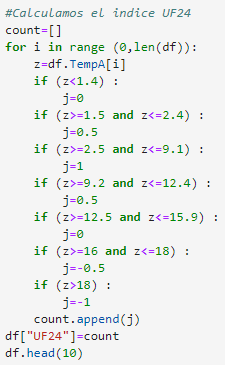
\includegraphics[scale = 0.65]{Images/uf24.png}
\end{center}

\section{Resultados}

\subsection{Evolución de las Temperaturas Máxima y Mínima}

\begin{center}
    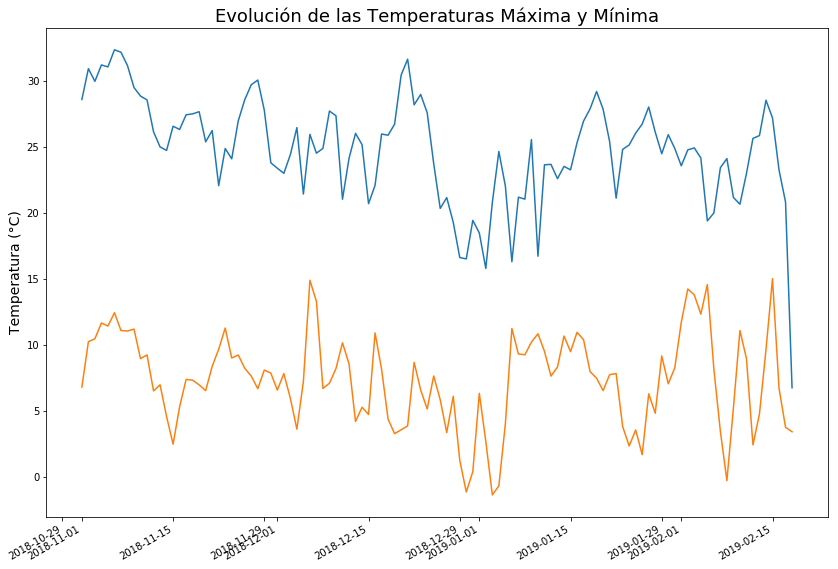
\includegraphics[scale = 0.40]{Images/GTemp.png}
\end{center}

\subsection{Acumulación de Horas Frío Desde el Primer Día}

\begin{center}
    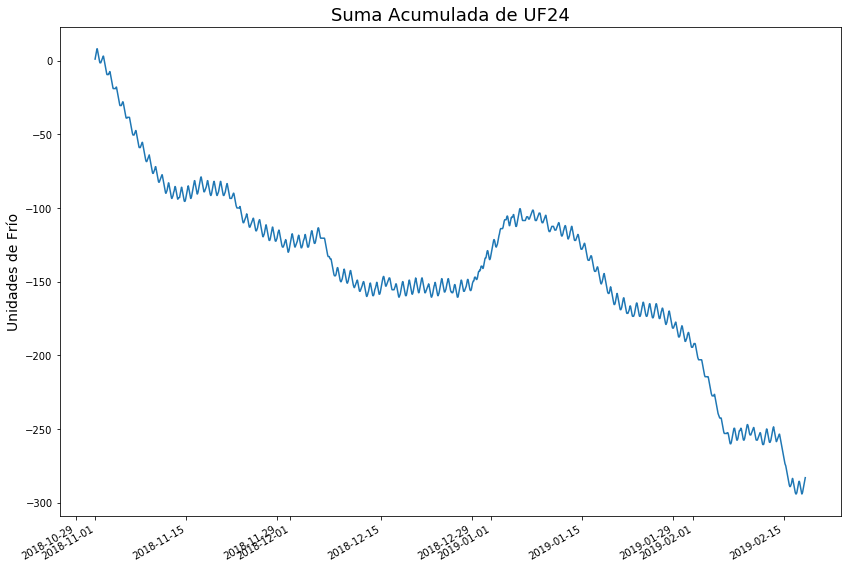
\includegraphics[scale = 0.44]{Images/GUF24.png}
\end{center}

\subsection{Modelo de INIFAP-CECH}
\noindent Se inician los cálculos desde principios de noviembre, cuando las temperaturas mínimas sean menores a 10ºC. Y se termina a finales de febrero. Se contará sólo cuando las Horas de Frío Efectivas sea positiva. 
\\

Se aplica el siguiente algoritmo:

HF = El número de horas frío por día (0 < T <= 10ºC)

HFE = El número de horas frío efectivas por día ( HFE = HF - número de horas con T >= 25ºC)
\subsubsection{Código}

\begin{center}
    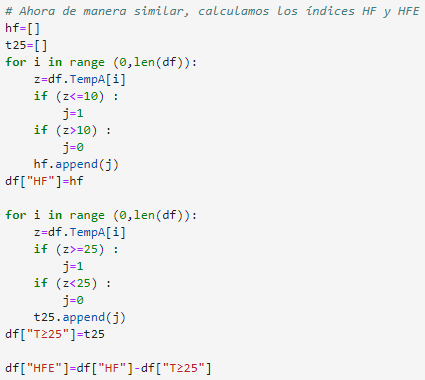
\includegraphics[scale = 0.73]{Images/HF.png}
\end{center}

\subsubsection{Gráfica}
\begin{center}
    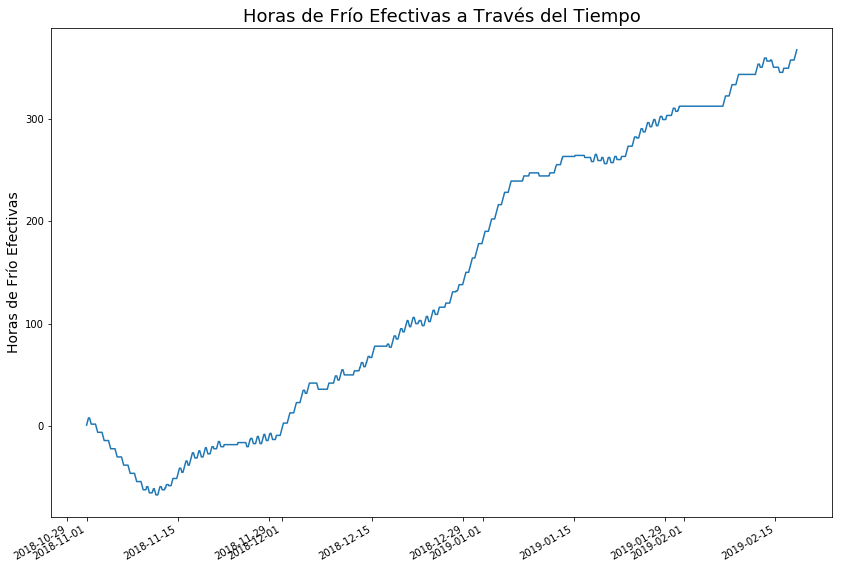
\includegraphics[scale = 0.4]{Images/GHF.png}
\end{center}

\subsection{Comparación}
\begin{center}
    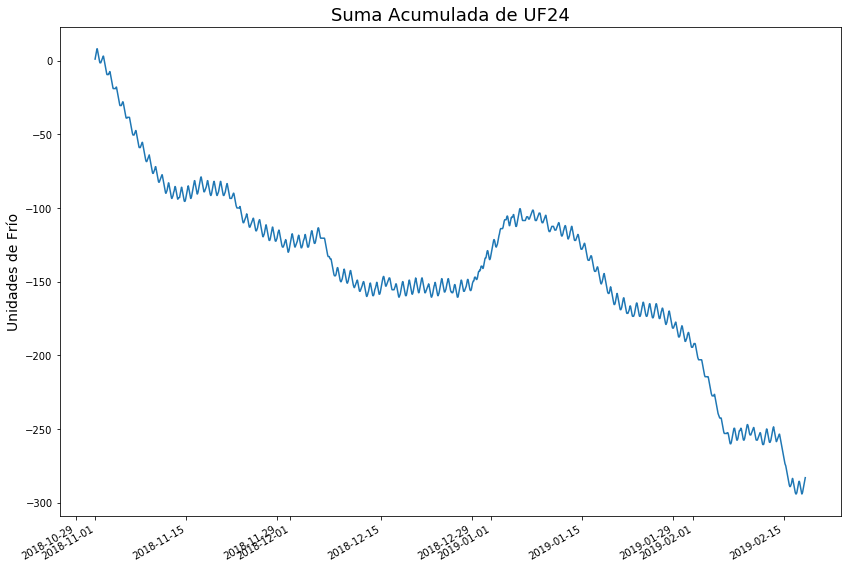
\includegraphics[scale = 0.25]{Images/GUF24.png}
    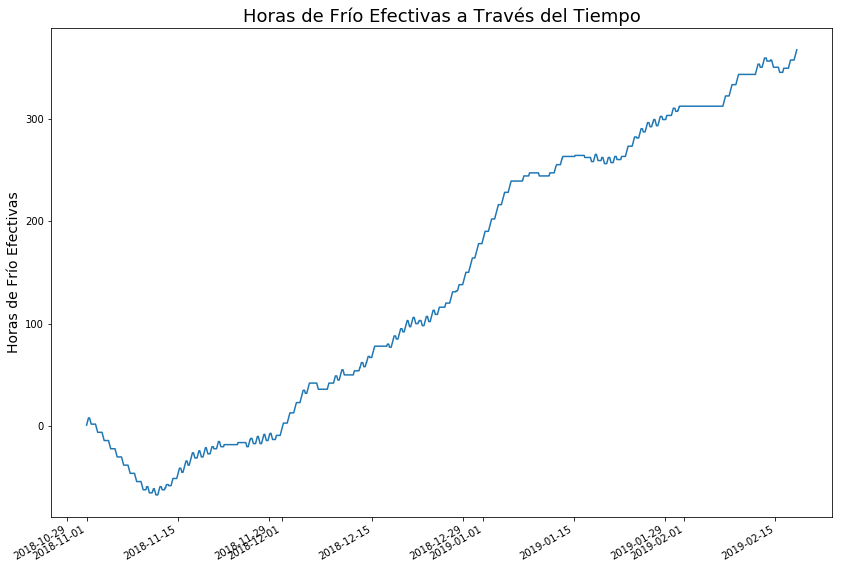
\includegraphics[scale = 0.25]{Images/GHF.png}
\end{center}
Donde se puede observar el comportamiento diferente de cada uno de los dos modelos. Esto indica que aunque se usen los mismos datos, el modelo cambia toda la perspectiva que teníamos.
\section{Conclusión}
A modo de conclusión, observando las gráficas generadas por las horas de frío acumuladas por día, podemos decir que lo que cambia el comportamiento es evidentemente el uso de diferentes modelos para calcular las unidades u horas de frío. También cabe resaltar que es importante hacer esto porque no todos los modelos se van a adaptar a todos los casos, aquí vimos que es necesario usar otro modelo, porque el frío de Sonora no es el mismo que en otras partes del planeta. Es por eso que el modelo Utah no es conveniente usarlo en estas regiones tan secas y cálidas.

\section{Bibliografía}

\begin{itemize}
    \item Requerimiento de frío en especies frutales caducifolias. (2009). Consultado el 08 de Marzo del 2019, de Wikipedia. Sitio web: 
    
    https://es.wikipedia.org/wiki/Requerimiento\_de\_fr\%C3\%ADo\_en\_especies\_frutales
    \_caducifolias\#Modelo\_de\_Utah
    
    \item Chill Calculators. (2019). Consultado el 08 de Marzo del 2019, de UCDAVIS Fruit \& Nuts Research \& Information. Sitio web:
    
    http://fruitsandnuts.ucdavis.edu/Weather\_Services/chilling\_accumulation\_models/Chill\_
    Calculators/index.cfm?step=form&type=chill&station=2
    
    
\end{itemize}


\end{document}
